\section{Introduction}
We use an example through the paper to illustrate 
the concepts.
Consider the network depicted in the figure \ref{fig:blacklist}.
In this network we have four switches and solid arrows show 
the initial routes.
Assume that two updates $p,q$ happen in the network.
The update $p$ replaces the route $cb$ with $cd$ and 
$q$ replaces the route $ab$ with $ac$.
Assume that the switch $d$ is blacklisted and as a result
existence of a path from $a$ to $d$ constitutes a safety 
violation.
Allowing both updates to happen in the network will result in the violation. 
In the following we show how we can use actual causality  
to capture this phenomenon as an actual case of the 
a safety property violation.

\begin{figure}
    \centering
    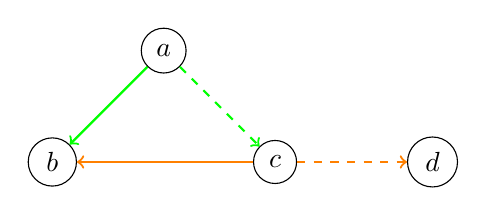
\begin{tikzpicture}[
            node distance={20mm},
            main/.style = {draw, circle},
            s/.style = {->,thick},
            d/.style = {->,thick,dashed} ]
        \node[main] (b) {$b$};
        \node[main] (a) [above right of=b] {$a$};
        \node[main] (c) [below right of=a] {$c$};
        \node[main] (d) [right of=c] {$d$};
        \draw[thick,green,->] (a) -- (b);
        \draw[thick,green,->,dashed] (a) -- (c);
        \draw[thick,orange,->] (c) -- (b);
        \draw[thick,orange,->,dashed] (c) -- (d);
    \end{tikzpicture}
    \caption{}
    \label{fig:blacklist}
\end{figure}